\documentclass[a4paper,addpoints]{exam}

\usepackage{commath}
\usepackage{siunitx}

% russian integral
\usepackage{scalerel}
\DeclareMathOperator*{\rint}{\scalerel*{\rotatebox{17}{$\!\int\!$}}{\int}}

\qformat{\textbf{\large{Question \thequestion}}\hfill}
\pointsinrightmargin
\boxedpoints

\begin{document}

\begin{coverpages}

\begin{center}
  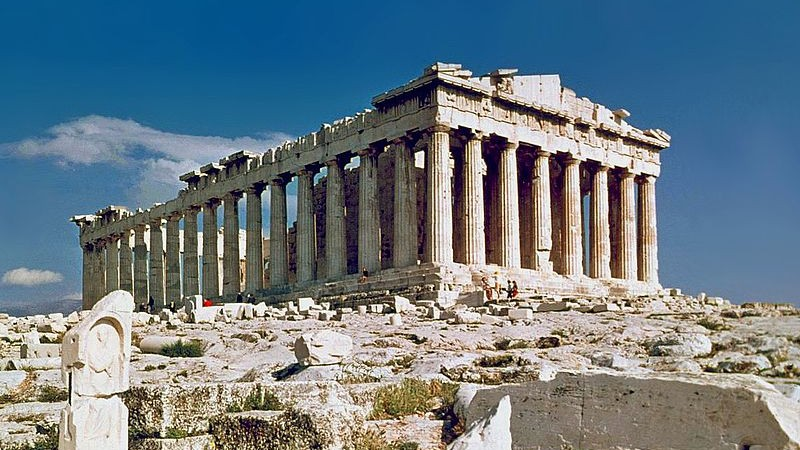
\includegraphics[width=0.6\textwidth]{exam-cover-04}

  \vspace{5mm}

  \textbf{\Huge{Level Three Calculus}}

  \vspace{2mm}

  \textbf{\Huge{Integration}}
\end{center}

\vspace{5mm}

\noindent
\large{There are three questions, worth a total of \numpoints\ marks.\\
       Attempt ALL questions, showing all working.\\
       Read questions carefully before attempting them.\\
       Marks are available for partial answers.\\
       The amount of time expected to be spent per question may not necessarily correlate ``nicely'' to the number of marks.\\
       Diagrams may be used to support answers.\\
       Candidates who do not provide diagrams for some questions may be disadvantaged.\\
       Some marks are given for clarity and neatness of solutions or proofs.}
\vspace{2mm}

\begin{tabular}{ll}
  \textbf{Time Allowed:}& One Hour\\
  \textbf{Achieved:}& 13 marks\\
  \textbf{Merit:}& 21 marks\\
  \textbf{Excellence:}& 29 marks
\end{tabular}

\vfill

\begin{center}
  \gradetable[h][questions]
  \vspace{2mm}

  \textbf{Available Grades:} \textit{Not Achieved}\quad\textit{Achieved}\quad\textit{Merit}\quad\textit{Excellence}
\end{center}

\end{coverpages}

\begin{questions}
  \question
    \begin{parts}
      \part Compute the following definite integrals.
        \begin{subparts}
          \subpart[2] $\displaystyle \rint^{\pi/2}_{\pi/4} 2\csc 2x \cot 2x \dif{x} $
          \subpart[2] $\displaystyle \rint^{4}_1 t \left( \frac{1.5}{\sqrt{t}} + 12 \right) \dif{t} $
        \end{subparts}
      \part[4] A balloon is being pumped up slowly such that its volume changes at a rate inversely proportional
            to the time $ t $ (in minutes); the rate can be modelled by $ \od{V}{t} = \frac{k}{t + 1} $ for some constant $ k $.
            The initial volume of the balloon was \SI{0.5}{\metre\cubed}, and after three minutes the volume had
            doubled. After what length of time will the volume of the balloon exceed \SI{2}{\metre\cubed}?
      \part[3] Find the area between the curves $ y = -\frac{1}{2}x^2 + \frac{3}{2}x $ and $ y = \frac{1}{2}x^2 - \frac{3}{2}x + 2 $ given
            that they intersect at $ (1,1) $ and $ (2,1) $.
    \end{parts}
  \question
    \begin{parts}
      \part Compute the following indefinite integrals.
        \begin{subparts}
          \subpart[1] $\displaystyle \rint \frac{2x + 1}{x^2 + x} \dif{x} $
          \subpart[3] $\displaystyle \rint \cos^4 \theta \dif{\theta} $
        \end{subparts}
      \part[3] Consider the functions $ f $ and $ g $ graphed in figure \ref{fig:nasty}. Given that the shaded region has a total area of 32 units squared,
            $ \rint^B_A f(x) - g(x) \dif{x} = 2 $, and $ \rint^D_C f(x) - g(x) \dif{x} = 10 $, compute
            \begin{displaymath}
              \rint^C_B f(x) - g(x) \dif{x}.
            \end{displaymath}
            \begin{figure}
              \centering
              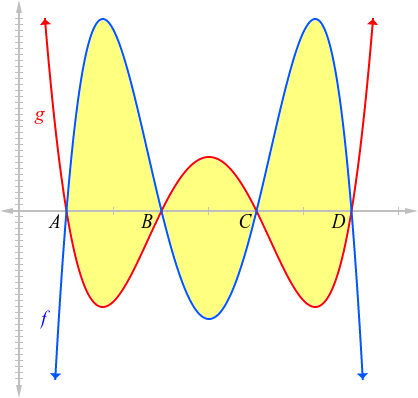
\includegraphics[width=0.5\textwidth]{nastyintegral}
              \caption{Two functions enclosing an area.\label{fig:nasty}}
            \end{figure}
      \part[4] Suppose that $ \od{y}{t} = (y + 1)(\sin 2\pi t) $, and $ y(0) = 1 $. Find $ y(0.5) $.
    \end{parts}

  \clearpage
  \question
    \begin{parts}
      \part[3] The \textit{volume of revolution} of a curve $ y = f(x) $ between two bounds $ x = a $ and $ x = b $
            is given by $ \pi\rint_a^b y^2 \dif{x} $. Find the volume of revolution of $ y = e^{-x} + 1 $ between $ x = 0 $ and $ x = 1 $
            by computing
            \begin{displaymath}
              \pi \rint^1_0 (e^{-x} + 1)^2 \dif{x}.
            \end{displaymath}
            The volume is visualised in figure \ref{fig:volrev}.
            \begin{figure}
              \centering
              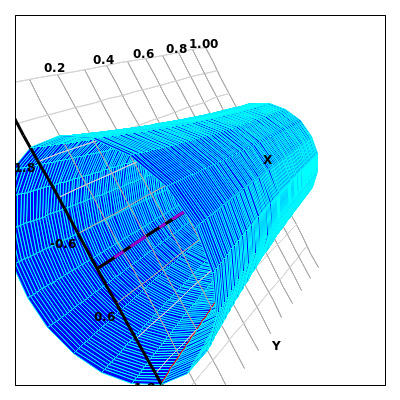
\includegraphics[width=0.5\textwidth]{volrev}
              \caption{The volume of revolution of $ e^{-x} + 1 $.\label{fig:volrev}}
            \end{figure}
      \part[3] Suppose that the acceleration of a particle is described at time $ t $ by the equation
            \begin{displaymath}
              \od[2]{x}{t} = 12t + 12.
            \end{displaymath}
            If the particle is initially located at $ x = 3 $, and is initially stationary, find the position
            of the particle at time $ t = 10 $.
      \part[4] Newton's law of cooling states that the rate of heat loss of an object is directly proportional to the difference in
            the temperatures between the object and its surroundings. Symbolically, if the environmental temperature is $ T_0 $, then
            \begin{displaymath}
              \od{T}{t} = -k(T - T_0).
            \end{displaymath}
            A loaf of bread is removed from an oven at a temperature of \SI{230}{\celsius}, and is left to cool in an
            area with a temperature of \SI{18}{\celsius}. How long, in terms of $ k $, will it take for the bread to cool to \SI{30}{\celsius}?
      \part[1] Explain why $ \rint_0^{2\pi} \tan x \dif{x} $ does not exist.
    \end{parts}
\end{questions}
\end{document}
